\documentclass[11pt,a4paper]{article}
\usepackage[margin=0.7in]{geometry}
\usepackage{amsmath,amssymb}
\usepackage{booktabs}
\usepackage{array}
\usepackage{graphicx}
\title{\textbf{E0 297: Cryptographic Hardware Accelerators} \\[4pt]
\Large Design Assignment 3: RSA-2048 Modular Exponentiation}
\author{Anirudh Chaturvedi \\ SR No: 25850}
\date{November 12, 2026}

\begin{document}
\maketitle

\section{Introduction \& Design Methodology}
This report presents the RTL design, microarchitecture, control/datapath state machines (FSM, FSMD, ASM, ASMD), design truth tables, functional verification, and ASIC synthesis of a parameterized RSA-2048 modular exponentiation core (\texttt{modexp \#(.N(2048))}) computing
\[
\text{modexp\_out} = \text{inp}^{\text{exp}} \bmod P
\]
using a \textbf{Left-to-Right Binary Square-and-Multiply} controller paired with a \textbf{Simple Interleaved Modular Multiplier} (\texttt{modmul}). The design is fully parameterized by bit-width $N$ and uses no optimizations specific to the RSA-2048 modulus $P$, making it applicable to any $N$-bit modulus.

\subsection{Top-Level Interface \& Input Pre-Reduction (\texttt{modexp.v})}
The top-level module preserves the exact required port list (\texttt{clock}, \texttt{write}, \texttt{reset} active-low synchronous, \texttt{start}, \texttt{ready}, \texttt{inp[N-1:0]}, \texttt{exp[N-1:0]}, \texttt{modexp\_out[N-1:0]}) and hardcoded 2048-bit modulus $P$:
\begin{itemize}
    \item \textbf{Input Latching (\texttt{write}):} On the rising clock edge where \texttt{write} is asserted, \texttt{inp} and \texttt{exp} are latched into \texttt{inp\_reg} and \texttt{exp\_reg}.
    \item \textbf{Modular Pre-Reduction (\texttt{start}):} Since Test Vectors 2, 4, and 5 in \texttt{inp\_2048.txt} have $\text{inp} \ge P$, \texttt{base} is reduced on \texttt{start} via \texttt{(inp\_reg >= P) ? (inp\_reg - P) : inp\_reg}. Because the MSB of $P$ is $1$, $\text{inp} < 2^N < 2P$, so a single conditional subtraction guarantees $0 \le \text{base} < P$.
    \item \textbf{Square-and-Multiply Controller:} Scanning \texttt{exp\_shift} from MSB ($N-1$) down to LSB ($0$), each bit performs $\text{res} \leftarrow (\text{res} \times \text{res}) \bmod P$, followed by $\text{res} \leftarrow (\text{res} \times \text{base}) \bmod P$ only if \texttt{exp\_shift[N-1] == 1}.
\end{itemize}

\subsection{Simple Interleaved Modular Multiplier (\texttt{modmul.v})}
Following Lecture 17 (Slide 11), \texttt{modmul} computes $(A \times B) \bmod P$ in $N$ clock cycles for $0 \le A, B < P$:
\begin{enumerate}
    \item Initialize $(N+2)$-bit accumulator $\texttt{acc} \leftarrow 0$ and shift register $\texttt{a\_reg} \leftarrow A$.
    \item Each cycle, compute $\texttt{acc\_shifted} = 2 \cdot \texttt{acc} + (\texttt{a\_reg}[N-1] \; ? \; B : 0)$, bounded by $3P$ ($N+2$ bits).
    \item Reduce modulo $P$ in one combinational step: subtract $2P$ if $\texttt{acc\_shifted} \ge 2P$, else subtract $P$ if $\texttt{acc\_shifted} \ge P$, else keep $\texttt{acc\_shifted}$.
\end{enumerate}

\clearpage
\section{Microarchitecture Block Diagram ($N = 2048$)}
Figure~\ref{fig:microarch} illustrates the complete hardware microarchitecture of \texttt{modexp} and \texttt{u\_modmul} using standard textbook datapath conventions: synchronous D-register blocks (with clock-edge triangles), 2:1 operand multiplexers, combinational modular arithmetic units, and dashed control paths.

\begin{figure}[h!]
\centering
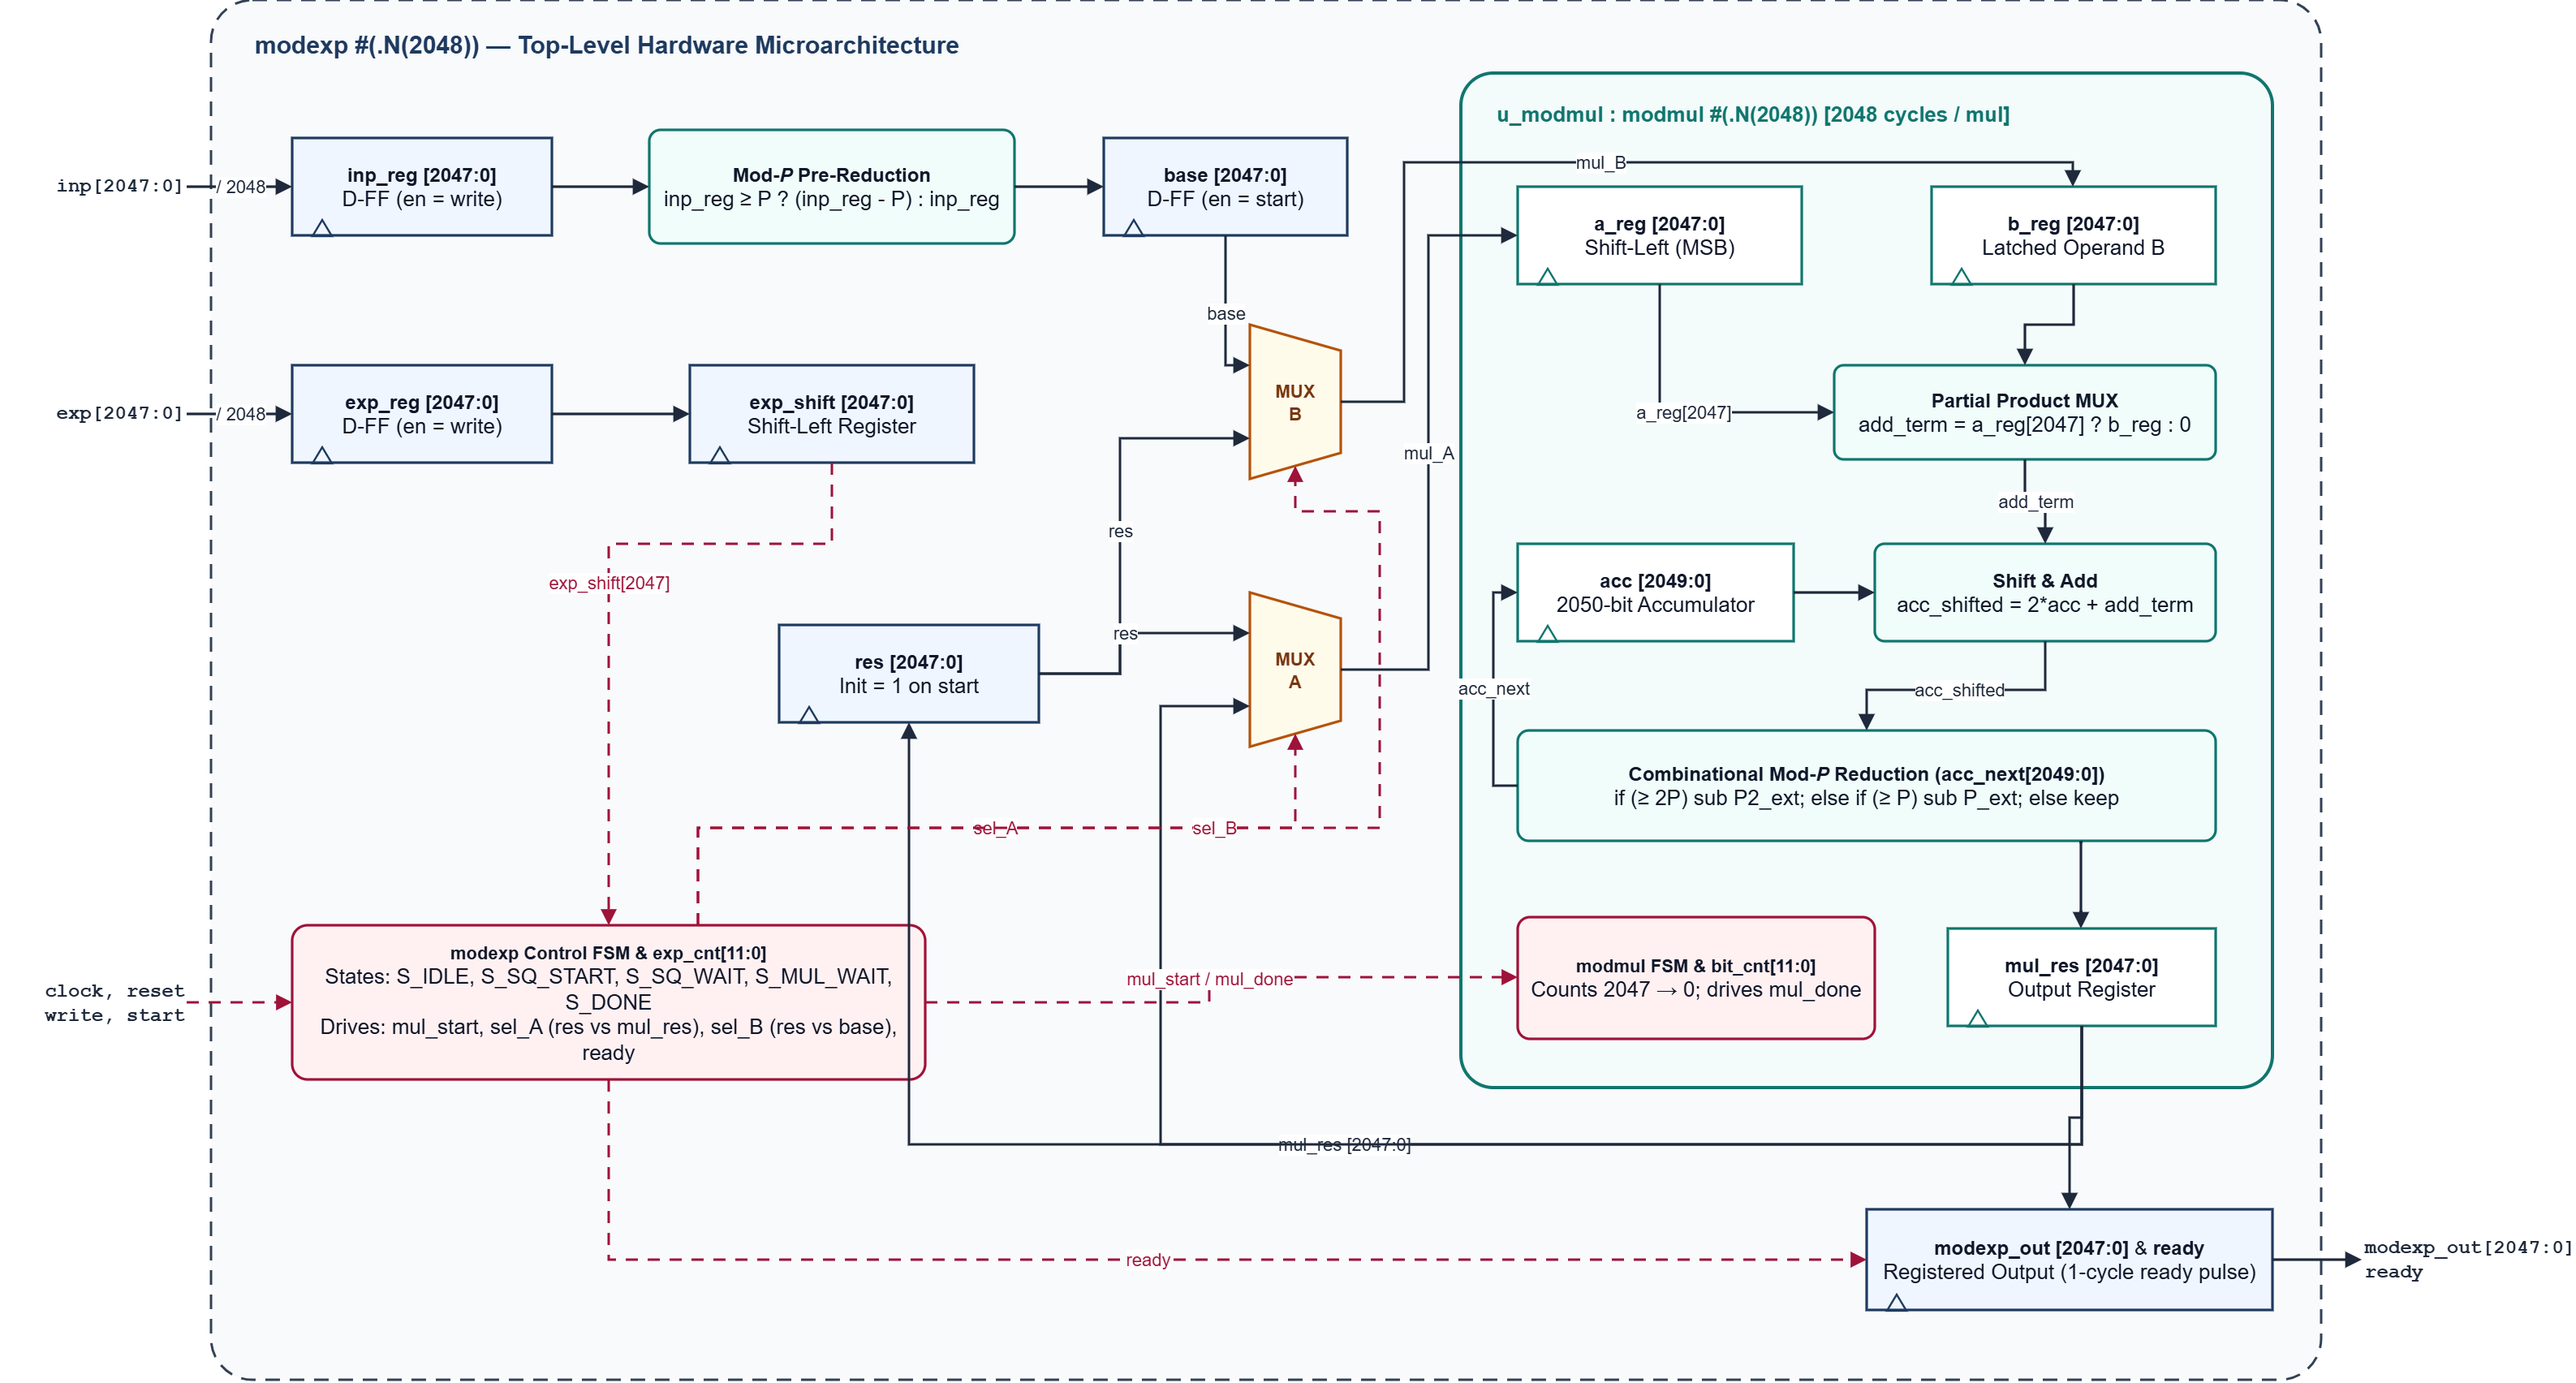
\includegraphics[width=\textwidth]{01_Microarchitecture.png}
\caption{Top-level hardware microarchitecture of \texttt{modexp \#(.N(2048))} and its internal \texttt{u\_modmul} interleaved modular multiplier.}
\label{fig:microarch}
\end{figure}

\clearpage
\section{Control FSM \& FSMD Diagrams}
Figure~\ref{fig:fsmd} presents the Finite State Machine with Datapath (FSMD) for both the 5-state top-level \texttt{modexp} controller and the 2-state \texttt{modmul} multiplier, showing exact state encodings, Mealy/Moore transitions, and RTL register transfers.

\begin{figure}[h!]
\centering
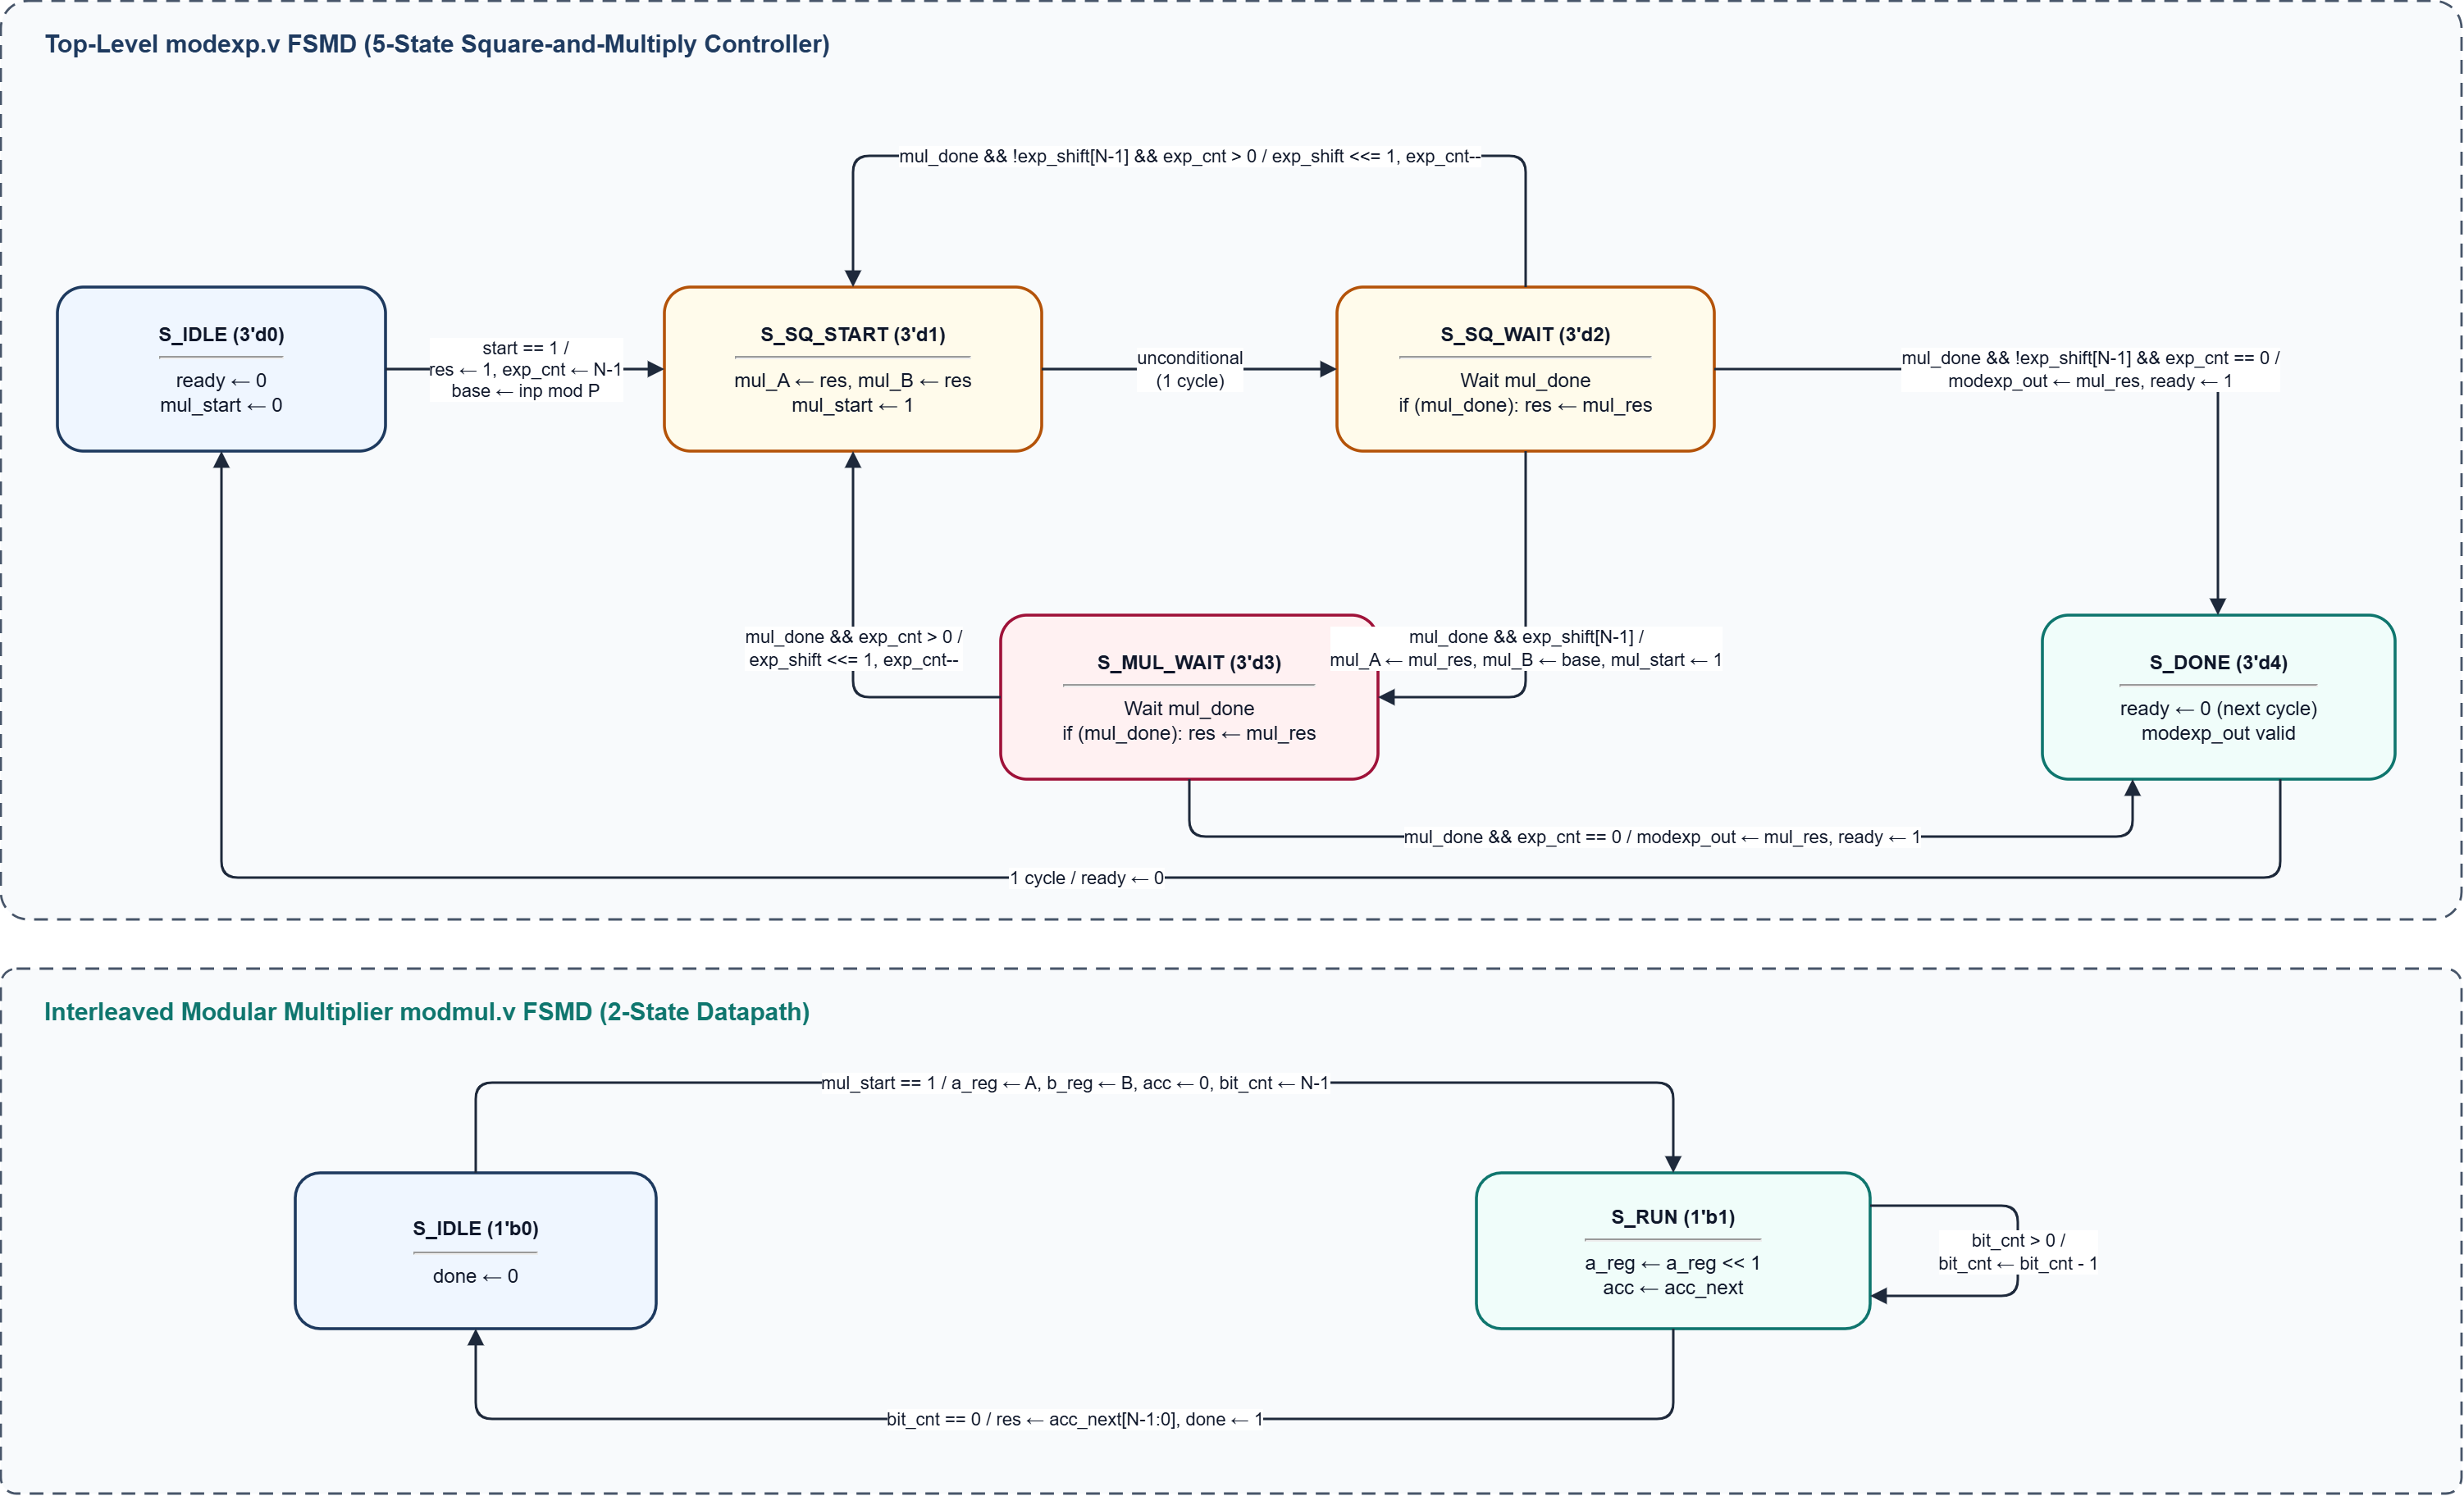
\includegraphics[width=\textwidth]{02_FSM_FSMD.png}
\caption{Control FSMD state transition diagrams for \texttt{modexp.v} (5 states) and \texttt{modmul.v} (2 states).}
\label{fig:fsm}
\end{figure}

\clearpage
\section{ASM \& ASMD Charts}
Figure~\ref{fig:asmd} presents the Algorithmic State Machine with Datapath (ASMD) charts using standard hardware notation: rectangular state boxes (navy), decision diamonds (amber), and rounded conditional RTL output boxes (teal).

\begin{figure}[h!]
\centering
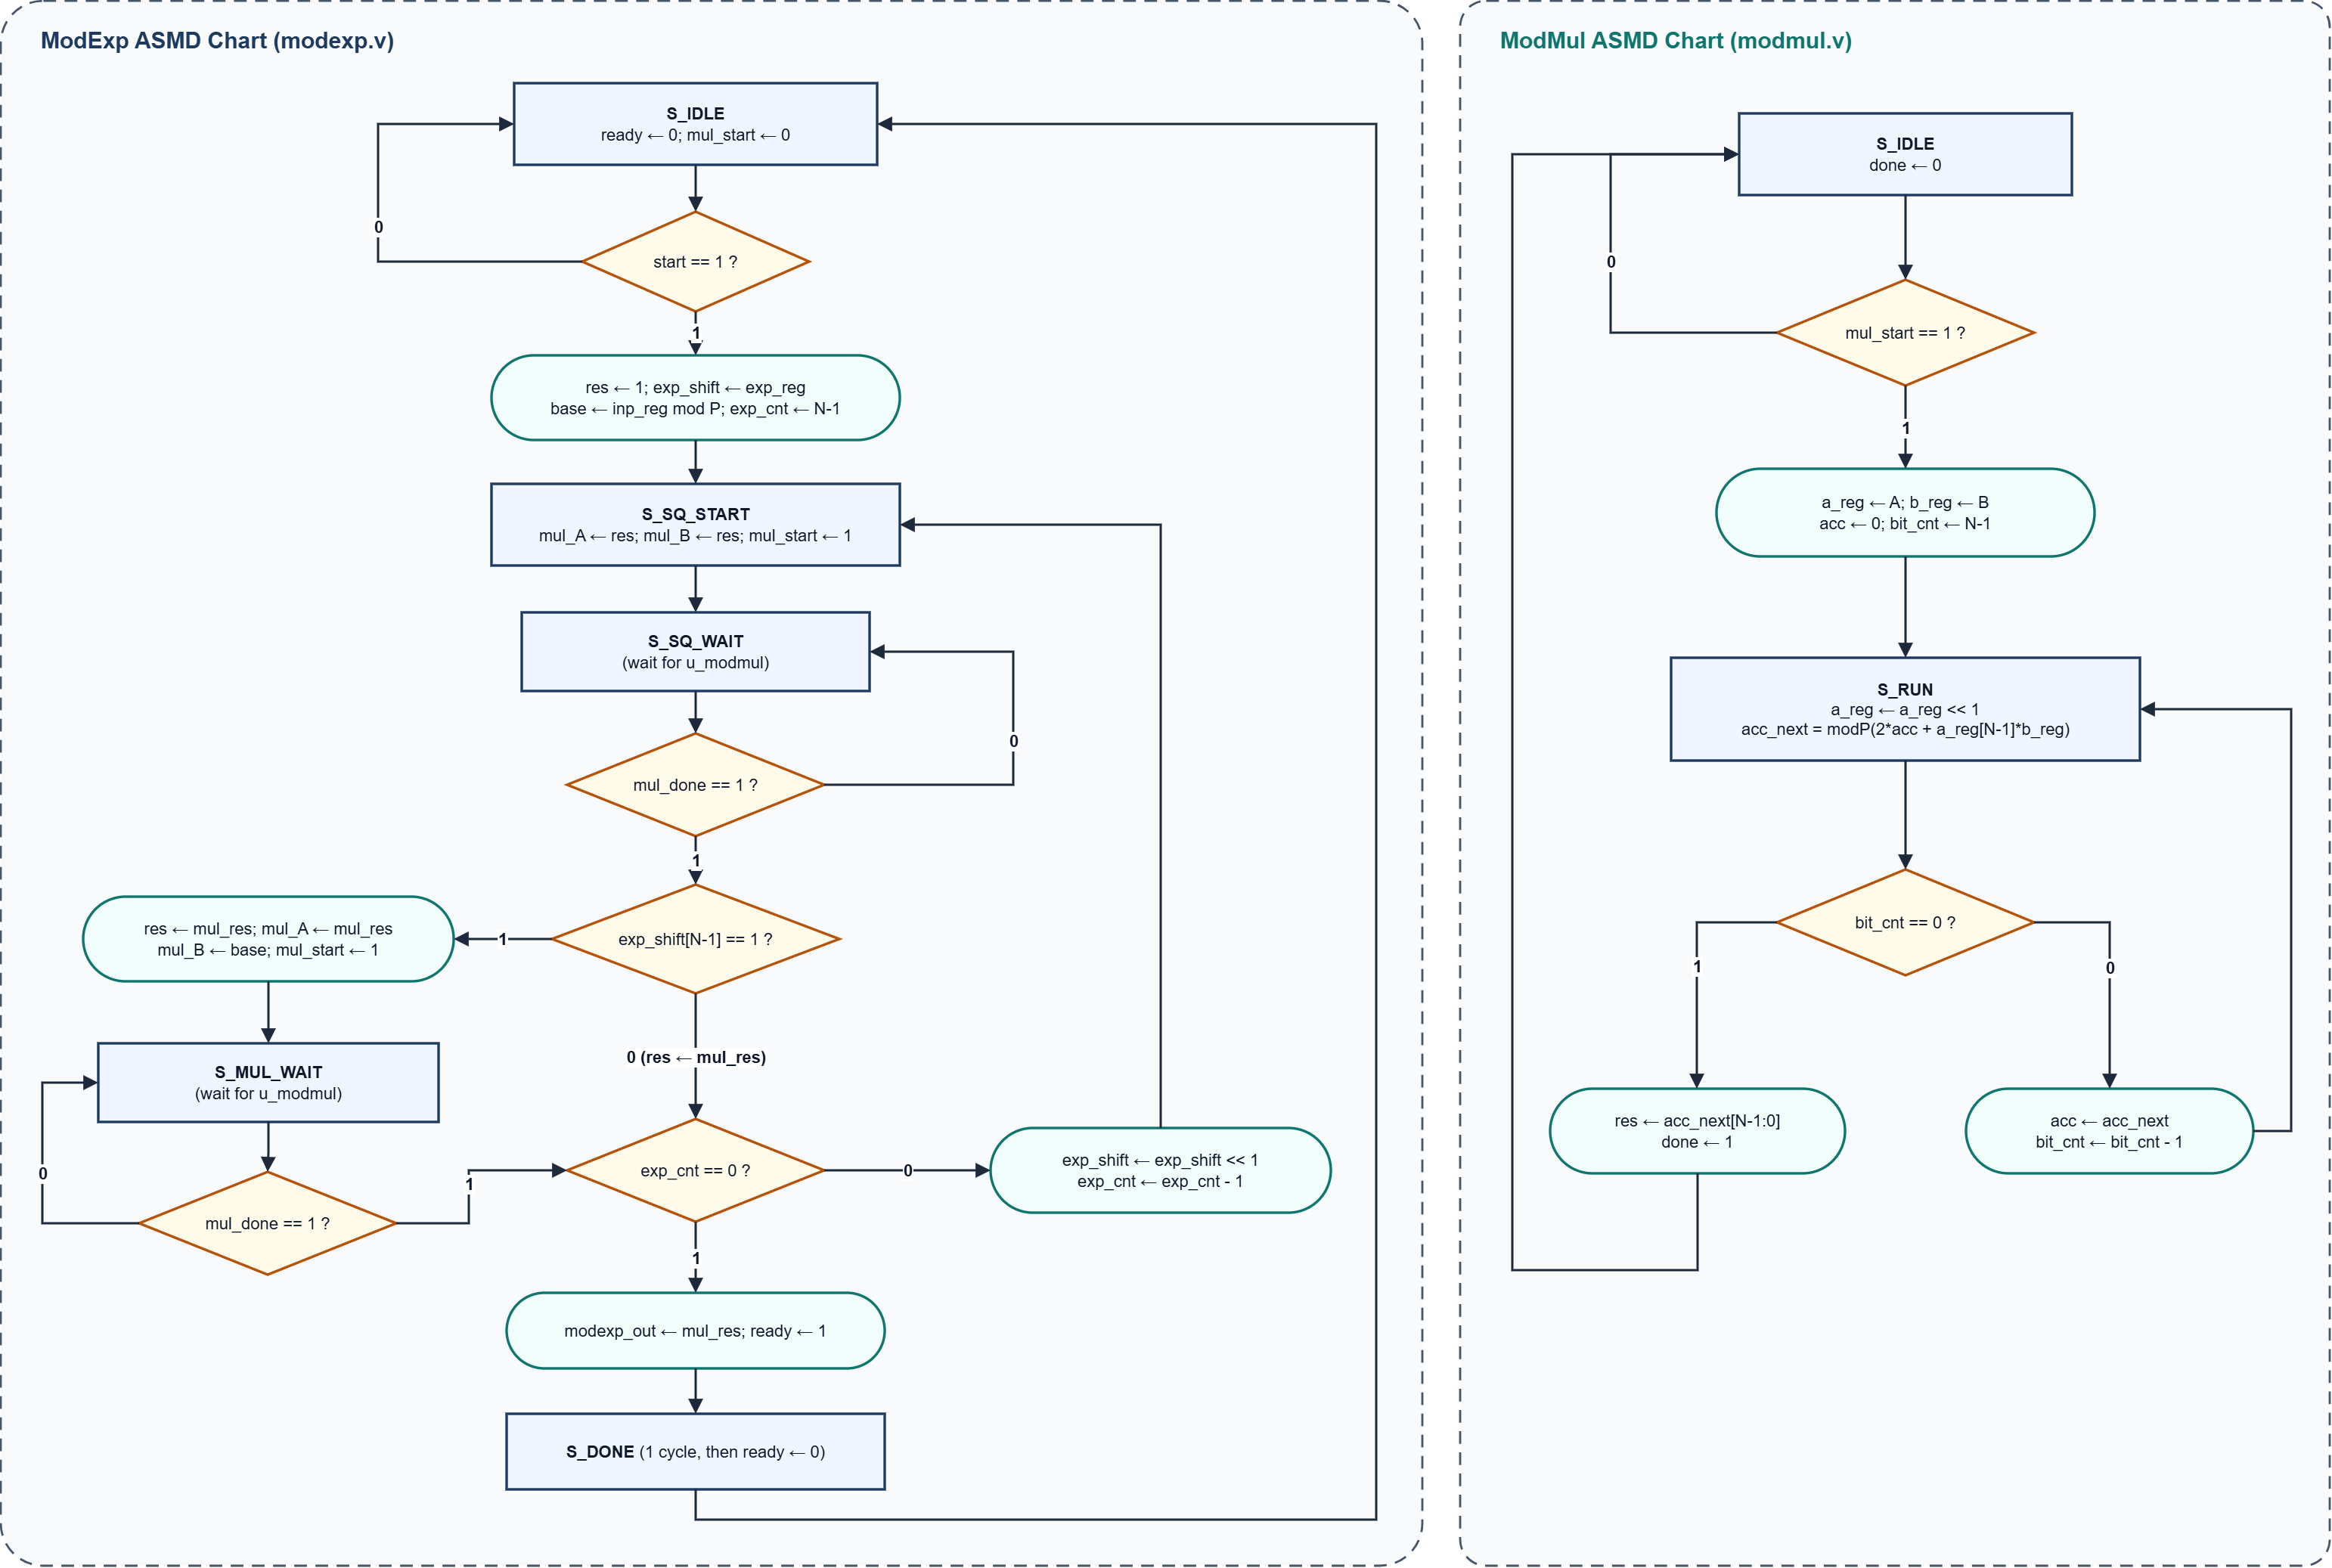
\includegraphics[width=\textwidth,height=0.82\textheight,keepaspectratio]{03_ASM_ASMD.png}
\caption{ASMD charts for \texttt{modexp.v} (left) and \texttt{modmul.v} (right), showing state boxes, decision diamonds, and conditional output ovals.}
\label{fig:asm}
\end{figure}

\clearpage
\section{Design Truth \& Control Tables}
Tables~\ref{tab:fsm_tt}, \ref{tab:red_tt}, and \ref{tab:mux_tt} specify the exact state-transition truth table, combinational modular reduction truth table, and operand multiplexer control logic used to synthesize the RTL.

\begin{table}[h!]
\centering
\caption{Top-Level \texttt{modexp} FSM State-Transition \& Output Truth Table}
\label{tab:fsm_tt}
\scriptsize
\begin{tabular}{@{}lp{3.6cm}lccp{3.6cm}@{}}
\toprule
\textbf{Current State} & \textbf{Condition} & \textbf{Next State} & \textbf{\texttt{mul\_start}} & \textbf{\texttt{ready}} & \textbf{Datapath Action} \\
\midrule
\texttt{ANY} & \texttt{reset == 0} & \texttt{S\_IDLE} & 0 & 0 & Clear all regs \\
\texttt{S\_IDLE} & \texttt{start == 0} & \texttt{S\_IDLE} & 0 & 0 & Hold idle \\
\texttt{S\_IDLE} & \texttt{start == 1} & \texttt{S\_SQ\_START} & 0 & 0 & \texttt{res}$\leftarrow$1, \texttt{base}$\leftarrow$\texttt{inp\_reg} mod $P$, \texttt{exp\_cnt}$\leftarrow N{-}1$ \\
\texttt{S\_SQ\_START} & \textit{unconditional} & \texttt{S\_SQ\_WAIT} & 1 & 0 & \texttt{mul\_A}$\leftarrow$\texttt{res}, \texttt{mul\_B}$\leftarrow$\texttt{res} \\
\texttt{S\_SQ\_WAIT} & \texttt{mul\_done == 0} & \texttt{S\_SQ\_WAIT} & 0 & 0 & Wait for \texttt{u\_modmul} \\
\texttt{S\_SQ\_WAIT} & \texttt{mul\_done \&\& exp\_shift[N-1]} & \texttt{S\_MUL\_WAIT} & 1 & 0 & \texttt{res}$\leftarrow$\texttt{mul\_res}, \texttt{mul\_A}$\leftarrow$\texttt{mul\_res}, \texttt{mul\_B}$\leftarrow$\texttt{base} \\
\texttt{S\_SQ\_WAIT} & \texttt{mul\_done \&\& !exp\_shift[N-1] \&\& exp\_cnt>0} & \texttt{S\_SQ\_START} & 0 & 0 & \texttt{res}$\leftarrow$\texttt{mul\_res}, \texttt{exp\_shift}$\ll=$1, \texttt{exp\_cnt--} \\
\texttt{S\_SQ\_WAIT} & \texttt{mul\_done \&\& !exp\_shift[N-1] \&\& exp\_cnt==0} & \texttt{S\_DONE} & 0 & 1 & \texttt{res}$\leftarrow$\texttt{mul\_res}, \texttt{modexp\_out}$\leftarrow$\texttt{mul\_res} \\
\texttt{S\_MUL\_WAIT} & \texttt{mul\_done == 0} & \texttt{S\_MUL\_WAIT} & 0 & 0 & Wait for \texttt{u\_modmul} \\
\texttt{S\_MUL\_WAIT} & \texttt{mul\_done \&\& exp\_cnt>0} & \texttt{S\_SQ\_START} & 0 & 0 & \texttt{res}$\leftarrow$\texttt{mul\_res}, \texttt{exp\_shift}$\ll=$1, \texttt{exp\_cnt--} \\
\texttt{S\_MUL\_WAIT} & \texttt{mul\_done \&\& exp\_cnt==0} & \texttt{S\_DONE} & 0 & 1 & \texttt{res}$\leftarrow$\texttt{mul\_res}, \texttt{modexp\_out}$\leftarrow$\texttt{mul\_res} \\
\texttt{S\_DONE} & \textit{unconditional} & \texttt{S\_IDLE} & 0 & 0 & Return to idle \\
\bottomrule
\end{tabular}
\end{table}

\begin{table}[h!]
\centering
\caption{Combinational Mod-$P$ Reduction Truth Table (\texttt{modmul.v})}
\label{tab:red_tt}
\small
\begin{tabular}{@{}ccc@{}}
\toprule
\textbf{\texttt{acc\_shifted >= 2P}} & \textbf{\texttt{acc\_shifted >= P}} & \textbf{Output \texttt{acc\_next[N+1:0]}} \\
\midrule
1 & X (1) & \texttt{acc\_shifted - P2\_ext} \\
0 & 1 & \texttt{acc\_shifted - P\_ext} \\
0 & 0 & \texttt{acc\_shifted} \\
\bottomrule
\end{tabular}
\end{table}

\begin{table}[h!]
\centering
\caption{Operand Multiplexer \& Pre-Reduction Control Table}
\label{tab:mux_tt}
\small
\begin{tabular}{@{}llll@{}}
\toprule
\textbf{Unit} & \textbf{Select Condition} & \textbf{Selected Input} & \textbf{Purpose} \\
\midrule
Pre-Reduction MUX & \texttt{inp\_reg >= P} (1 / 0) & \texttt{inp\_reg - P} / \texttt{inp\_reg} & Enforce $0 \le \text{base} < P$ \\
Operand B MUX & State (\texttt{S\_SQ\_START} / \texttt{S\_SQ\_WAIT}) & \texttt{res} / \texttt{base} & Square vs.\ Multiply \\
\texttt{modmul} Bit MUX & \texttt{a\_reg[N-1]} (1 / 0) & \texttt{b\_reg} / \texttt{0} & Partial product \texttt{add\_term} \\
\bottomrule
\end{tabular}
\end{table}

\clearpage
\section{Functional Verification}
The RTL (\texttt{modexp.v}, \texttt{modmul.v}) was simulated against the unmodified testbench \texttt{modexp\_tb.v} and all 10 golden 2048-bit test vectors using \textbf{Verilator 5.032}. All \textbf{10 / 10 test cases PASSED} with zero failures and zero timeouts.

\begin{table}[h!]
\centering
\caption{Per-Vector Cycle Count and Verification Summary ($N = 2048$)}
\small
\begin{tabular}{@{}ccccc@{}}
\toprule
\textbf{Test Vector} & \textbf{$\text{inp} < P$} & \textbf{Exp Hamming Weight} & \textbf{Clock Cycles} & \textbf{Status} \\
\midrule
1 & Yes & 1005 & 6,254,594 & PASS \\
2 & No ($\text{inp} \ge P$) & 1001 & 6,246,402 & PASS \\
3 & Yes & 982 & 6,207,490 & PASS \\
4 & No ($\text{inp} \ge P$) & 1082 & 6,412,290 & PASS \\
5 & No ($\text{inp} \ge P$) & 1016 & 6,277,122 & PASS \\
6 & Yes & 1026 & 6,297,602 & PASS \\
7 & Yes & 1026 & 6,297,602 & PASS \\
8 & Yes & 1021 & 6,287,362 & PASS \\
9 & Yes & 1010 & 6,264,834 & PASS \\
10 & Yes & 1005 & 6,254,594 & PASS \\
\midrule
\textbf{Average} & --- & \textbf{1017.4} & \textbf{6,279,989.2} & \textbf{10/10 PASS} \\
\bottomrule
\end{tabular}
\end{table}

\section{ASIC Synthesis, Timing, Power \& Energy Results}
Synthesis was performed using \textbf{Yosys 0.52} and static timing/power analysis using \textbf{OpenSTA 3.1.0} with \texttt{NangateOpenCellLibrary\_typical.lib} (using \texttt{BUF\_X1} driving cell and \texttt{10.0} load constraint).

\begin{table}[h!]
\centering
\caption{RSA-2048 \texttt{modexp} ASIC Implementation Metrics (Nangate 45nm Typical)}
\small
\begin{tabular}{@{}lp{0.55\textwidth}@{}}
\toprule
\textbf{Metric} & \textbf{Measured Value} \\
\midrule
Total Standard Cells & 143,730 \\
Total Chip Area & $240,591.41\;\mu\text{m}^2$ \\
Sequential Area & $111,277.38\;\mu\text{m}^2$ (46.25\%) \\
Combinational Area & $129,314.04\;\mu\text{m}^2$ (53.75\%) \\
\midrule
Clock Cycles (Min / Avg / Max) & 6,207,490 / 6,279,989.2 / 6,412,290 \\
Critical Path Delay ($T_{\min}$) & 20.6742 ns (arrival 20.6355 ns + setup 0.0387 ns) \\
Maximum Clock Frequency ($f_{\max}$) & \textbf{48.37 MHz} \\
Hold Slack (Min Path) & +0.0287 ns (MET) \\
\midrule
Power @ 100 MHz (10.0 ns) & 43.80 mW (Internal: 29.5 mW, Switching: 9.30 mW, Leakage: 4.99 mW) \\
Power @ $f_{\max}$ (48.37 MHz) & 23.76 mW (Dynamic: 18.77 mW, Leakage: 4.99 mW) \\
Average Latency @ $f_{\max}$ & 129.83 ms \\
Energy per RSA-2048 ModExp @ $f_{\max}$ & \textbf{3.085 mJ} \\
\bottomrule
\end{tabular}
\end{table}

\end{document}
